
\setcounter{chapter}{2}
\chapter{System Design and Architecture}
\minitoc %insert la minitoc
\graphicspath{{Chapitre3/figures/}}

%\DoPToC
%==============================================================================
\pagestyle{fancy}
\fancyhf{}
\fancyhead[R]{\bfseries\rightmark}
\fancyfoot[R]{\thepage}
\renewcommand{\headrulewidth}{0.5pt}
\renewcommand{\footrulewidth}{0pt}
\renewcommand{\chaptermark}[1]{\markboth{{\chaptername~\thechapter. #1 }}{}}
\renewcommand{\sectionmark}[1]{\markright{\thechapter.\thesection~ #1}}

\begin{spacing}{1.2}

%==============================================================================
\section*{Introduction}
This chapter presents the system design and architecture of the LLM-powered best practices enforcement system. Building on the business understanding and requirements established in the previous chapter, this chapter details the technical design decisions, architectural patterns, and system components that enable real-time, intelligent feedback for YouTube framework development.

The design follows traditional software engineering principles while incorporating modern AI technologies. This chapter covers the overall system architecture, component design, data models, and integration patterns that form the foundation of the implemented solution.

\section{System Architecture Overview}


\subsection{Use Case Analysis}

Understanding the system's interactions with its users is fundamental to designing an effective solution. The use case analysis identifies the primary actors and their interactions with the LLM Best Practices Enforcement System, establishing the scope and boundaries of the system's functionality.

\begin{figure}[H]
\centering
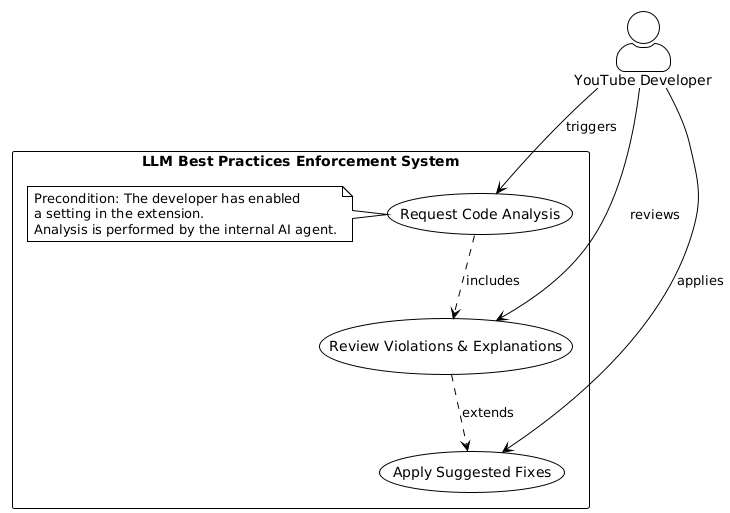
\includegraphics[scale=0.6]{images/use_case_diagram.png}
\caption{System Use Case Diagram}
\label{fig:use_case_diagram}
\end{figure}

This use case diagram illustrates the core functionality of the system from the perspective of YouTube developers. The primary actor is the YouTube Developer, who interacts with the system through three main use cases: requesting code analysis, reviewing violations and explanations, and optionally applying suggested fixes. The relationship between use cases reflects the natural workflow: analysis always includes reviewing results, while applying fixes is an optional extension that developers can choose based on their needs and preferences. This design ensures that developers maintain control over their workflow while providing comprehensive feedback when requested. The diagram focuses on the most important scenarios that occur during normal system usage, avoiding authentication and administrative scenarios that are less central to the user experience.


\subsection{High-Level Architecture}
The system architecture is designed to integrate seamlessly into the developer's existing workflow while providing intelligent, context-aware feedback. The architecture consists of two main components that work together to deliver real-time best practice enforcement:

\begin{itemize}
    \item \textbf{IDE}: The developer's workspace containing the YouTube IDE Extension, which works with the currently open file being analyzed and annotates results directly in the editor.
    \item \textbf{AI Agent Framework}: The processing layer containing the LLM Best Practices Agent, which serves as the core AI processing engine that uses internal LLMs to analyze code and suggest best practices.
\end{itemize}

\begin{figure}[H]
\centering
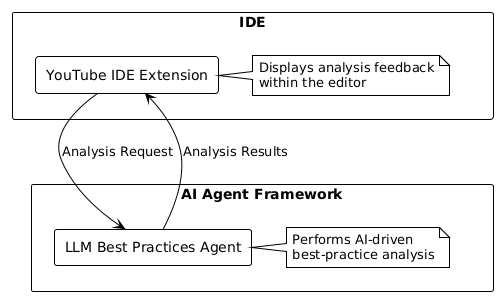
\includegraphics[scale=0.7]{images/high_level_system_architecture.png}
\caption{High-Level System Architecture}
\label{fig:system_architecture}
\end{figure}

This architecture diagram illustrates the fundamental separation between the user-facing IDE extension and the AI processing backend. The YouTube IDE Extension operates within the developer's workspace, providing immediate access to analysis capabilities while maintaining the familiar development environment. The AI Agent Framework handles the computationally intensive analysis tasks, ensuring that the IDE remains responsive during processing. This separation enables independent scaling of AI capabilities without impacting the development environment's performance.

\subsection{System Workflow}
The system operates through a streamlined workflow that begins when a developer triggers analysis via the YouTube IDE Extension. The complete interaction flow is depicted in Figure \ref{fig:sequence_diagram}.

\begin{figure}[H]
\centering
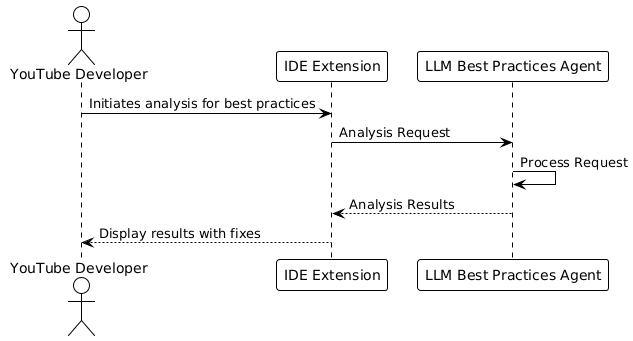
\includegraphics[scale=0.7]{images/sequence_diagram.png}
\caption{System Interaction Sequence Diagram}
\label{fig:sequence_diagram}
\end{figure}

This sequence diagram captures the most important interaction scenario: a developer requesting analysis of their current file. The diagram shows the complete flow from user action to result presentation, demonstrating how the system maintains responsiveness by delegating heavy processing to the AI agent while providing immediate feedback through the IDE extension. This represents the primary use case that occurs most frequently in the system.

The sequence unfolds through the following interactions and responsibilities:
\begin{enumerate}
    \item \textbf{Analysis initiation}: The YouTube developer triggers analysis of the currently open file.
    \item \textbf{Request submission}: The YouTube IDE Extension submits an analysis request to the agent, identifying the target file.
    \item \textbf{Processing}: The agent performs best-practices analysis and prepares the resulting findings.
    \item \textbf{Result delivery}: The agent returns a structured response to the YouTube IDE Extension.
    \item \textbf{Presentation}: The YouTube IDE Extension presents the best practices violations and suggested fixes within the editor.
\end{enumerate}

This workflow emphasizes decoupling the IDE from heavy AI computation, ensuring that the development environment remains responsive while delegating intensive analysis to the specialized agent framework.

\section{Components Design}

\subsection{LLM Best Practices Agent} 
The LLM Best Practices Agent serves as the core intelligence engine of the system, responsible for analyzing code, identifying violations of YouTube framework best practices, and providing actionable feedback to developers. This component represents the convergence of modern AI capabilities with domain-specific software engineering expertise.

\subsubsection{Agent Architecture Choice}
The agent is built using the \textit{Executable Agent} architecture~\cite{microsoftAgentPatterns}, provided by our internal AI platform. This architecture offers a structured approach to orchestrating AI-powered workflows, and was selected after careful evaluation of different agent paradigms, considering reliability, performance, and maintainability.

\paragraph{Executable Agent vs. ReAct Architecture}
To motivate the choice of \textit{Executable Agent} architecture, we contrast it with the more widely known ReAct (Reasoning and Acting) pattern. In our system, the \textit{Executable Agent} refers to a deterministic, tool-orchestrated workflow where control flow is defined in code rather than delegated to LLM reasoning.

\begin{itemize}
    \item \textbf{ReAct Agent}: Uses a reasoning loop where the LLM decides what action to take next, executes it, observes the result, and continues reasoning. This creates a dynamic, LLM-driven execution flow.
    \item \textbf{Executable Agent}: Follows a predefined, deterministic execution flow where the agent orchestrates a sequence of tool calls in a structured manner, with the LLM used primarily for processing within each tool rather than for orchestration decisions.
\end{itemize}


Figure~\ref{fig:agent_comparison} illustrates the fundamental difference in control flow between the two approaches.

\begin{figure}[H] 
	\centering 
	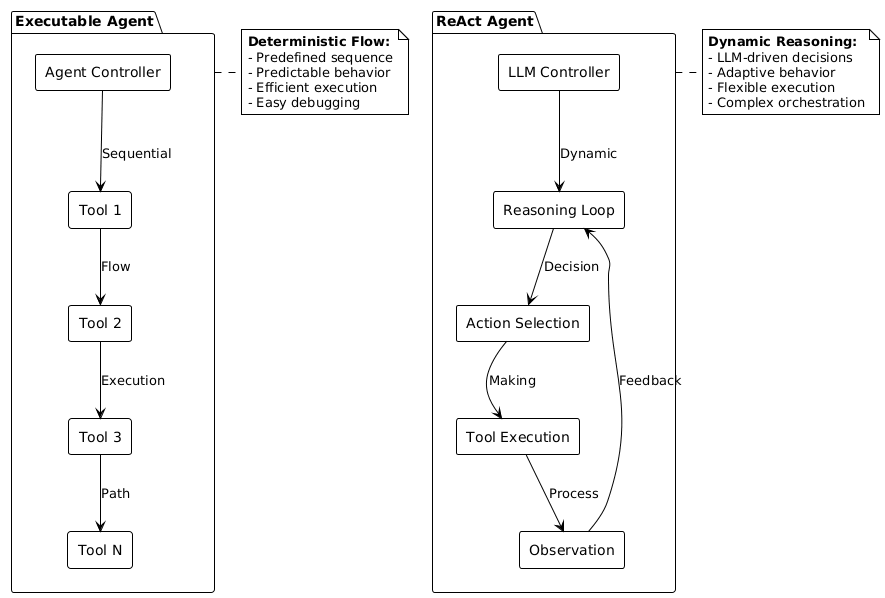
\includegraphics[scale=0.6]{images/agent_architecture_comparison.png} 
	\caption{Comparison of Executable Agent vs. ReAct Agent Architectures} 
	\label{fig:agent_comparison} 
\end{figure}

The Executable Agent architecture offers several key advantages for this use case:
\begin{itemize}
    \item \textbf{Deterministic Execution}: Predefined flow ensures predictable behavior and simplifies debugging.
    \item \textbf{Tool Orchestration}: Clean framework for coordinating multiple specialized tools.
    \item \textbf{Error Handling}: Built-in mechanisms for handling failures and graceful degradation.
    \item \textbf{Performance}: Efficient execution with low response latency, since orchestration decisions are pre-programmed rather than deferred to open-ended LLM reasoning.
    \item \textbf{Cost Efficiency}: Reduced token consumption by constraining LLM calls to focused, well-scoped processing steps rather than repeated reasoning loops.
    \item \textbf{Maintainability}: Clear separation of concerns between tools and responsibilities.
\end{itemize}



\subsubsection{Core Tools Architecture}
To achieve this structured workflow, the agent incorporates five specialized tools, each handling a specific step of the best practices analysis pipeline.

\paragraph{Tool Responsibilities}
The agent's tool architecture follows a sequential workflow where each tool has a distinct responsibility:

\begin{itemize}
    \item \textbf{File Reading Tool}: Responsible for retrieving the complete content of the file being analyzed, ensuring the agent has access to the full context of the code under examination.
    
    \item \textbf{Code Analysis Tool}: The core analysis engine that performs violation detection against YouTube framework best practices using semantic code analysis to understand intent and context.
    
    \item \textbf{Violation Explanation Tool}: Generates human-readable explanations for each identified violation, providing developers with clear understanding of why particular code patterns violate best practices.
    
    \item \textbf{Code Fix Tool}: Proposes actionable fix suggestions for identified violations, going beyond problem identification to provide concrete solutions that developers can implement.
    
    \item \textbf{Result Consolidation Tool}: Aggregates all analysis results into a structured output format, ensuring the response contains all necessary information for the IDE extension to display results effectively.
\end{itemize}

This tool-based architecture provides clear separation of concerns, with each tool handling a specific aspect of the analysis pipeline while maintaining a cohesive workflow. 
\subsubsection{Processing Strategy}
The agent employs a balanced processing strategy that weighs performance against reliability. This strategy represents a key architectural decision made after evaluating different processing approaches for handling multiple violations within a single file.

\paragraph{Processing Strategy Options}
During the design phase, three main processing strategies were considered for handling multiple violations:

\begin{itemize}
    \item \textbf{Fully Sequential Processing}: Each violation is processed one at a time, ensuring maximum reliability and predictability but potentially resulting in longer processing times for files with many violations.
    
    \item \textbf{Fully Parallel Processing}: All violations are processed concurrently, maximizing performance but introducing complexity in managing concurrent operations and potential reliability challenges under high load conditions.
    
    \item \textbf{Hybrid Processing Strategy}: A balanced approach that processes violations efficiently while maintaining system stability. This strategy provides significant performance improvements over sequential processing while ensuring reliable operation under various load conditions.
\end{itemize}

The hybrid processing strategy was selected as it provides the optimal balance between performance and reliability for production use. This strategy ensures that the agent can handle complex analysis tasks efficiently while maintaining system stability and providing consistent results.

\subsubsection{Integration with LLM Infrastructure}
The agent integrates with an internal AI platform that hosts multiple LLM models. The architecture is model‑agnostic, enabling seamless adoption of newer models as they are released without requiring changes in the orchestration logic. LLM usage is isolated behind stable interfaces so higher‑level logic remains unaffected. The analysis tools depend on the LLM for semantic understanding and code generation. This design ensures long‑term maintainability and benefits from platform improvements without architectural change.

\subsection{YouTube IDE Extension}
The YouTube IDE Extension serves as the user-facing interface that seamlessly integrates the LLM Best Practices Agent into YouTube developers' daily workflow. Since YouTube developers are the primary target audience for this system, the YouTube IDE Extension was chosen as the natural entry point, leveraging their existing development environment and workflow patterns. This component is designed to provide intelligent, context-aware feedback while maintaining the responsiveness and familiarity that developers expect from their development environment. The feature becomes available when developers enable a user setting in the extension, and entry points only appear for files that belong to the internal YouTube framework for which we enforce best practices.

\subsubsection{Extension Architecture}
The YouTube IDE Extension serves as a lightweight client that orchestrates the interaction between developers and the AI analysis system. The architecture ensures responsiveness by delegating computationally intensive analysis to the specialized agent framework while handling user interface concerns, progress indication, and result presentation locally.

\subsubsection{User-Triggered vs. Automatic Analysis Design Decision}
A fundamental design decision for the IDE extension was whether to implement user-triggered analysis or automatic analysis. This choice significantly impacts user experience, system performance, and resource utilization.

The primary motivation for user-triggered analysis stems from the need to maintain developer productivity and system efficiency. LLM analysis is computationally expensive and resource-intensive, making continuous analysis impractical for maintaining IDE responsiveness. User-triggered analysis ensures that analysis occurs only when developers specifically request it, providing contextually relevant feedback at optimal moments without interrupting their workflow. This approach aligns with developer expectations of having control over their development environment while ensuring that computational resources are used efficiently.

Table \ref{tab:analysis_approaches} summarizes the trade-offs:

\begin{table}[H]
\centering
\caption{Comparison of User-Triggered vs. Automatic Analysis Approaches}
\label{tab:analysis_approaches}
\begin{tabular}{|l|c|c|}
\hline
\textbf{Criteria} & \textbf{User-Triggered} & \textbf{Automatic} \\
\hline
User Control & $\checkmark$ & $\times$ \\
\hline
Resource Efficiency & $\checkmark$ & $\times$ \\
\hline
IDE Performance & $\checkmark$ & $\times$ \\
\hline
Contextual Timing & $\checkmark$ & $\times$ \\
\hline
Discoverability & $\times$ & $\checkmark$ \\
\hline
Always Current & $\times$ & $\checkmark$ \\
\hline
\end{tabular}
\end{table}

Based on this analysis, the user-triggered approach was selected as it provides superior resource management, user control, and system performance. The trade-offs in discoverability and stale state management are addressed through intuitive UI design and comprehensive feedback mechanisms.

\paragraph{Stale State Challenge}
The user-triggered approach introduces a fundamental design challenge: maintaining the relevance and accuracy of analysis results as developers continue modifying their code. This challenge requires balancing system responsiveness with result accuracy, ensuring that feedback remains useful throughout the development process.

\subsubsection{User Interface Design}
The YouTube IDE Extension is designed around two core interaction patterns: entry points for initiating analysis and feedback mechanisms for presenting results.

\paragraph{Entry Points}
The YouTube IDE Extension provides multiple entry points to ensure accessibility and discoverability for different user preferences and workflows:

\begin{itemize}
    \item \textbf{Visual Interface Integration}: Visual indicators are integrated into the development environment to provide immediate visibility of AI analysis availability, ensuring maximum discoverability while maintaining a clean interface.
    
    \item \textbf{Command-Based Access}: For developers who prefer keyboard-driven workflows, the extension provides command-based access through standard IDE navigation patterns, supporting both mouse-driven and keyboard-driven user interactions.
\end{itemize}

\paragraph{Feedback Mechanisms}
The YouTube IDE Extension employs three core feedback mechanisms designed to integrate seamlessly with existing development workflows:

\begin{itemize}
    \item \textbf{Progress Indication}: Real-time status updates during analysis processing to maintain developer awareness and system transparency.
    
    \item \textbf{Violation Display}: Presentation of analysis results using familiar interface patterns that leverage developers' existing knowledge of standard feedback mechanisms.
    
    \item \textbf{Contextual Suggestions}: Interactive code solutions that appear when developers interact with violation markers, providing actionable recommendations.
\end{itemize}


\subsubsection{User Interaction Flow}
The user interaction flow with the YouTube IDE Extension follows a structured pattern from analysis initiation to optional fix application:

\begin{figure}[H]
\centering
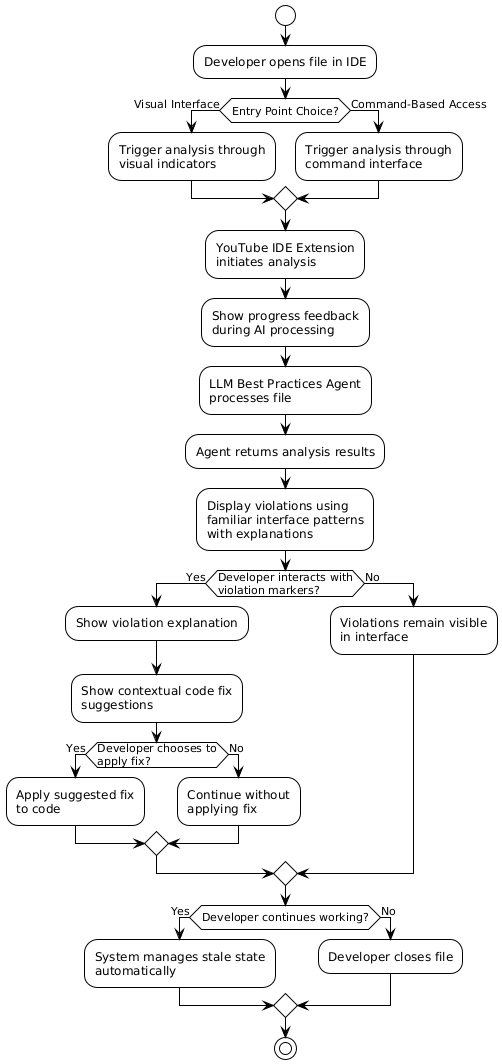
\includegraphics[scale=0.6]{images/user_flow.png}
\caption{YouTube IDE Extension User Interaction Flow: Complete developer journey from analysis trigger to fix application}
\label{fig:user_interface_flow}
\end{figure}

The flow demonstrates the core interaction pattern: developers initiate analysis through visual or command interfaces, receive progress feedback during processing, and interact with displayed violations to access explanations and optional fixes. This design ensures developers maintain control over their workflow while providing comprehensive feedback when requested.


\section{Data Models and Interfaces}

\subsection{Input/Output Specification}
The system's data models define the contracts between components, ensuring consistent communication and data exchange throughout the analysis pipeline. These interfaces establish clear boundaries between the IDE extension and the AI agent, enabling independent evolution of each component.

\paragraph{Analysis Request Format}
The YouTube IDE Extension sends analysis requests to the LLM Best Practices Agent using a minimal input format that identifies the target file for analysis. This design choice ensures that the agent can focus on its core responsibility of code analysis while maintaining security and proper workspace isolation. The request format includes the file path.

\paragraph{Analysis Response Format}
The agent returns a structured response containing the analysis results, error information, and optional metadata. The response format includes status information indicating success or failure, violation details with explanations and suggested fixes, and usage statistics for monitoring purposes. This standardized format ensures that the IDE extension can consistently process and display results regardless of the underlying analysis complexity.

\subsection{Convention Data Management}
The system's convention data model defines how YouTube framework best practices are structured, stored, and accessed throughout the analysis pipeline.

\paragraph{Convention Data Structure}
The convention data model captures best practice definitions as structured objects that support efficient programmatic access and analysis. Each convention definition includes essential metadata such as unique identifiers, descriptions, correct examples, and incorrect examples. This structure enables rapid lookup and context-specific retrieval during code analysis, with the design optimized for constant-time access patterns required by the agent's processing pipeline.

\paragraph{Storage Architecture Decision}
The system employs an in-memory storage approach using structured Python objects rather than external file-based or database storage. This design decision balances several architectural considerations:

\begin{itemize}
    \item \textbf{Data Characteristics}: Conventions are static during runtime, requiring no dynamic updates, making in-memory storage appropriate for performance-critical analysis.
    \item \textbf{Performance Requirements}: In-memory access ensures ultra-low-latency retrieval for real-time analysis, eliminating I/O overhead during agent execution.
    \item \textbf{Simplicity \& Reliability}: Structured Python objects provide type safety and eliminate parsing overhead while ensuring data integrity.
    \item \textbf{Resource Efficiency}: Conventions are loaded once at startup, minimizing runtime resource consumption and avoiding repeated file system access.
    \item \textbf{Architectural Flexibility}: The design allows future migration to external storage if multi-framework support or dynamic updates become necessary.
\end{itemize} 

\paragraph{Integration Interfaces}
The system defines minimal, versioned boundaries that keep components decoupled:

\begin{itemize}
    \item \textbf{IDE Extension Interface}: Contract between the YouTube IDE Extension and the LLM Best Practices Agent that defines the analysis request and response format, enabling independent evolution of UI and agent components.
    \item \textbf{Convention Access Interface}: Defines how the agent accesses convention definitions through in-memory lookup mechanisms, providing a stable boundary for data retrieval without external dependencies.
    \item \textbf{Monitoring Interface}: Captures usage statistics and performance metrics for system observability and evaluation purposes.
\end{itemize}


\subsection*{Conclusion}
The architecture of the LLM Best Practices Agent is defined by three central design decisions. First, the adoption of the Executable Agent paradigm ensures deterministic execution, structured tool orchestration, and predictable performance, avoiding the drawbacks of open-ended reasoning loops. Second, the hybrid parallel–sequential processing strategy balances efficiency with interpretability, allowing analyses to scale while maintaining transparency in intermediate results. Finally, the IDE extension provides a seamless developer experience, integrating feedback, explanations, and fixes directly into familiar workflows while managing state and staleness automatically. Together, these pillars create a robust, cost-efficient, and developer-friendly system for embedding AI-driven best practice enforcement into the coding environment.
%==============================================================================
\end{spacing}
